\documentclass[10pt,letterpaper]{article}
\usepackage[top=0.85in,left=2.75in,footskip=0.75in]{geometry}

\usepackage{listings}
\usepackage[T1]{fontenc}

% amsmath and amssymb packages, useful for mathematical formulas and symbols
\usepackage{amsmath,amssymb}

% Use adjustwidth environment to exceed column width (see example table in text)
\usepackage{changepage}

% Use Unicode characters when possible
\usepackage[utf8x]{inputenc}

% textcomp package and marvosym package for additional characters
\usepackage{textcomp,marvosym}

% cite package, to clean up citations in the main text. Do not remove.
\usepackage{cite}

% Use nameref to cite supporting information files (see Supporting Information section for more info)
\usepackage{nameref,hyperref}

% line numbers
\usepackage[right]{lineno}

% ligatures disabled
\usepackage{microtype}
\DisableLigatures[f]{encoding = *, family = * }

% color can be used to apply background shading to table cells only
\usepackage[table]{xcolor}

% array package and thick rules for tables
\usepackage{array}

% create "+" rule type for thick vertical lines
\newcolumntype{+}{!{\vrule width 2pt}}

% create \thickcline for thick horizontal lines of variable length
\newlength\savedwidth
\newcommand\thickcline[1]{%
  \noalign{\global\savedwidth\arrayrulewidth\global\arrayrulewidth 2pt}%
  \cline{#1}%
  \noalign{\vskip\arrayrulewidth}%
  \noalign{\global\arrayrulewidth\savedwidth}%
}

% \thickhline command for thick horizontal lines that span the table
\newcommand\thickhline{\noalign{\global\savedwidth\arrayrulewidth\global\arrayrulewidth 2pt}%
\hline
\noalign{\global\arrayrulewidth\savedwidth}}


% Remove comment for double spacing
%\usepackage{setspace}
%\doublespacing

% Text layout
\raggedright
\setlength{\parindent}{0.5cm}
\textwidth 5.25in
\textheight 8.75in

% Bold the 'Figure #' in the caption and separate it from the title/caption with a period
% Captions will be left justified
\usepackage[aboveskip=1pt,labelfont=bf,labelsep=period,justification=raggedright,singlelinecheck=off]{caption}
\renewcommand{\figurename}{Fig}

% Use the PLoS provided BiBTeX style
\bibliographystyle{plos2015}

% Remove brackets from numbering in List of References
\makeatletter
\renewcommand{\@biblabel}[1]{\quad#1.}
\makeatother



% Header and Footer with logo
\usepackage{lastpage,fancyhdr,graphicx}
\usepackage{epstopdf}
%\pagestyle{myheadings}
\pagestyle{fancy}
\fancyhf{}
%\setlength{\headheight}{27.023pt}
%\lhead{\includegraphics[width=2.0in]{PLOS-submission.eps}}
\rfoot{\thepage/\pageref{LastPage}}
\renewcommand{\headrulewidth}{0pt}
\renewcommand{\footrule}{\hrule height 2pt \vspace{2mm}}
\fancyheadoffset[L]{2.25in}
\fancyfootoffset[L]{2.25in}
\lfoot{\today}

%\titlerunning{Null models for Network Enrichment Analysis}
%\authorrunning{G. S. Jeuken and L. K\"{a}ll}

%\Copyright{Gustavo S. Jeuken and Lukas K\"{a}ll}%mandatory, please use full first names. LIPIcs license is "CC-BY";  http://creativecommons.org/licenses/by/3.0/


\begin{document}
\vspace*{0.2in}

% Title must be 250 characters or less.
\begin{flushleft}
{\Large
\textbf\newline{A simple null model for inferences from network enrichment analysis} % Please use "sentence case" for title and headings (capitalize only the first word in a title (or heading), the first word in a subtitle (or subheading), and any proper nouns).
}
\newline
% Insert author names, affiliations and corresponding author email (do not include titles, positions, or degrees).
\\
Gustavo S. Jeuken\textsuperscript{1} and
Lukas K\"{a}ll\textsuperscript{1,*}
\\
\bigskip
\textbf{1} Science for Life Laboratory, School of Engineering Sciences in Chemistry, Biotechnology and Health, KTH -- Royal Institute of Technology, Box 1031, 17121 Solna, Sweden
\\
\bigskip

% Use the asterisk to denote corresponding authorship and provide email address in note below.
*lukas.kall@scilifelab.se
\end{flushleft}
% Please keep the abstract below 300 words
\section*{Abstract}
A prevailing technique to infer function from lists of identifications, from molecular biological high-throughput experiments, is over-representation analysis, where the identifications are compared to predefined sets of related genes often referred to as pathways. As at least some pathways are known to be incomplete in their annotation, algorithmic efforts have been made to complement them with information from functional association networks. While the terminology varies in the literature, we will here refer to such methods as Network Enrichment Analysis (NEA). Traditionally, the significance of inferences from NEA has been assigned using parametric models, that are tuned by fitting parameters by sampling random network perturbations. Here we instead have designed one dynamic programming algorithm that calculates the score distribution of NEA scores and makes it possible to assign unbiased mid $p$~values to inferences. We also implemented a random sampling method, carrying out the same task. We demonstrate that our method obtains a superior statistical calibration as compared to the popular NEA inference engine, BinoX, while also providing statistics that are easier to interpret.



\section*{Introduction}

Over-Representation Analysis (ORA) is commonly used to infer function from sets of analytes such as genes, transcripts, proteins or metabolites\cite{tavazoie1999systematic,khatri2012ten,goeman2007analyzing}. The technique estimates which functional modules, such as complexes or pathways, are overrepresented among a set of identified analytes. One prominent application of the technique is expression analysis, where ORA is regularly used to assess alternation in pathway activity by examining significantly different concentrations of analytes between biological conditions, such as disease state or treatment group.

Most ORA methods are assessing the overlap between the investigated set of analytes, the {\em query set}, and a functional module, the {\em pathway set}, using hypergeometric test or a Fisher's exact test. However, variants such as Gene Set Enrichment Analysis (GSEA)\cite{subramanian2005gene} also includes information on expression levels of the analytes of the query set.

A limiting factor of ORA is the quality of the databases defining pathways. While \url{http://pathguide.org} list 708 databases of pathway definitions\cite{bader2006pathguide},  some critique has been voiced concerning the completeness and rigor of current pathway databases. Hence efforts have been directed to designing methods that extend the pathway definitions, by functional association networks, like STRING\cite{szklarczyk2014string} and FunCoup\cite{ogris2017funcoup}. Instead of directly examining the overlap between the query and pathway sets, one can evaluate the number of links in the functional association network that connect the query and pathway set\cite{alexeyenko2012network, glaab2012enrichnet, mccormack2013statistical, ogris2016novel, signorelli2016neat}. While the terminology varies in the literature, we will here refer to such methods as {\em Network Enrichment Analysis} (NEA).

The significance of the inferences from NEA is assessed by null models that investigate the number of expected random links from the query gene set to the pathway. Previous efforts have settled for various parametric null distributions, where the parameters are estimated by Monte Carlo-simulations that permute the network definitions by methods with varying degrees of topological conservation.

% As the often used network randomization techniques are not completely random, such methods often introduce an undesirable bias in the statistics. For instance, the actual set of random networks is much larger than the ones one use in such test, namely the random networks that retain a certain topological characteristic\cite{newman2001random}. 
% Also, the somewhat inaccessible process used to randomize networks produces statistics that are equally hard to interpret, as such statistic in practice test a more complex null model than intended.
The methods that are used for network randomization, while computationaly efficient, are often mentally untractable as they include a big number of steps that are subject to complex constrains.
As an example, in the link assignment plus second-order conservation method \cite{mccormack2013statistical}, links are assigned at random, but sequentially and at each step they must follow contrains that essentially depends on all previous steps.
And so, while in the end we do come to a network that is randomized while preserving some desired topological features, the nested constrains make it very hard to describe the probability space to which this network belongs. 
We will then come to a null hypothesis for which rejection is uninformative, defeating the purpose the statistical test.

Users of NEA typically want to test if there is a functional association between a query set of genes and a pathway\cite{alexeyenko2012network}. We argue that such test is much easier implemented as tests of the query set, i.e. is the query set a randomly selected set of genes or is there an over representation of well-connected genes in the query set?

Hence, here we employ a different null model, more directly aimed at modeling the lack of association between query and pathway gene sets, which we formulate as ``there are not more links between the query and pathway gene sets than expected by chance''. We present a dynamic programming algorithm, that we dubbed GeneSetDP, that calculates the exact score distribution of any query of a given size, noting here that we do not need to make any assumptions on the nature of the score distribuition. We also implemented one random sampling algorithm for the same task, that we called GeneSetMC.
The algorithms enabled us to calculate well-defined statistics of inferences from NEA that we argue is more intuitive from an end-user perspective and thus more likely to be interpreted in a correct manner.
Using simulations we demonstrated that both the algorithms produced unbiased statistics.

\section*{Algorithms}

In network-based gene set analysis one scores a query set of genes, $ \mathcal{Q}=\{g_1 \ldots g_Q\}$, from a genome with genes, $\mathcal{G}=\{g_1 \ldots g_G\}$ (i.e. $\mathcal{Q} \subseteq \mathcal{G}$), and how they relate to a pathway, $\mathcal{P}=\{p_1 \ldots p_P\}$. In NEA the pathway maps to the genome through a network, ${x_{ij}}$, where $x_{ij}=1$ if $g_i$ and $p_j$ are connected, or $x_{ij}=0$ otherwise. The pathways are scored by summing up all connections, i.e. the pathway score can be expressed as,

\begin{equation}
s=\sum_{i=1}^Q\sum_{j=1}^P x_{ij}.
\label{eq:sum_ij}
\end{equation}

We wanted to evaluate our score under the null hypothesis, $H_0$ : ``There are not more links between the query and pathway gene sets than expected by chance''. This formulation translates to calculating the distribution of scores that would occur if the $Q$ query genes are randomly selected from the genome, and see how frequently a score as extreme or more extreme than the current score would appear in that distribution. Hence, we wanted to determine a score distribution, {\em i.e.} the number of ways, $N(s)$, we can pick $Q$ genes and obtain a score, $s$, which we will give two methods for below. Given such a score distribution, we can express a mid $p$~value\cite{lancaster1961significance,hwang2001optimality} for obtaining a score, $s$, as,

\begin{equation}
p(s)=\frac{N(s)/2 +\sum_{s'=s+1}^{S} N(s')}{\sum_{s'=0}^{S} N(s')},
\label{eq:pval}
\end{equation}
where $S$ is the maximal score, $s$, that $Q$ genes can obtain from Eq~(\ref{eq:sum_ij}).

We can reformulate Eq~(\ref{eq:sum_ij}) by defining the number of links, $l_i=\sum_{j=1}^P x_{ij}$, which gives us a score,
\begin{equation}
s=\sum_{i=1}^Q l_i.
\label{eq:sum_i}
\end{equation}
Such number of links, $l_i$, can be pre-computed for all genes in $\mathcal{G}$. For later purposes we also define a mapping, $k_a=\sum_{\{i:l_i=a\}}1$, giving the number of genes having $a$ links to the investigated pathway.



\subsection*{Random sampling algorithm}

We first implemented a random sampling algorithm to assess $N(s)$. We randomly selected sets of $Q$ genes from $\mathcal{G}$. These sets scores were calculated with Eq~(\ref{eq:sum_i}). We counted the number of times, $F_B(s)$, a score of $s$ was obtained when sampling $B$ gene sets. We see that $F_B(s)$ will approximately have the same shape as $N(s)$ when selecting a large $B$, and we can hence calculate $p$~values by replacing $N$ with $F_B$ in Eq~(\ref{eq:pval}). We refer to this procedure as GeneSetMC.

\subsection*{Computation of the score distribution}

An alternative approach is to calculate the exact score distribution using dynamic programming. This can be done if we formulate $N(s)$ as a recursion, by observing a partial sum function,  $N_a(s,c)$,
 which expresses the number of ways to select a set of $c$ query genes, each with $\le a$  links to the pathway set and obtain a score of $s$. If we know the distribution of the number of ways to select genes with $\le a-1$ genes,  $N_{a-1}(s,c)$, for all $s$ and $c$,   $N_a(s,c)$ can be determined by investigating the ways to select genes with exactly $a$ links to the investigated pathway.   As there are $k_a \choose b$ ways to select $b$ from $k_a$ elements, there contribution to $N_a(s,c)$ from the selection of  $b$ genes with exactly $a$ links are ${k_a \choose b} N_{a-1}(s-ab,c-b)$. When evaluating all possible values of $b$ we see that
 \begin{equation}
N_a(s,c)=\sum_{b=0}^{k_a}{k_a \choose b} N_{a-1}(s-ab,c-b).
\end{equation}
We also see that $N_a(s,c)=0$ for all $s<0$, $c<0$ or $a<0$, with the exception of $N_{-1}(0,0)=1$.

The final score distribution is given by $N(s)=N_R(s,Q)$, where $R=\max_{i}{l_i}$, i.e the largest number of links to the pathway from any gene in the genome.


\subsection*{Implementation}

\begin{lstlisting}[language=Python, caption={ The central part of the dynamic programing algorithm for finding $N(s)$. The function takes the vector of links per gene, $k_a$, as well as the number of query genes, $Q$ as an input. The function depends on two additional functions {\tt find\_maxscore(k,Q)}, which calculates the maximal score a query of size $Q$ can obtain, and {\tt comb(a,b)}, which calculates $ a \choose b $.}, label=lst:gensetdp, captionpos=t, float, abovecaptionskip=-\medskipamount]
def genesetdp(k,Q):
    max_s = find_maxscore(k,Q)
    N = np.zeros((max_s+1,Q+1))
    N[0,0] = 1

    for a in range(len(k)):
        for s in range(max_s,-1,-1):
            for c in range(Q,-1,-1):
                for b in range(k[a],0,-1): # Stop at b=1
                    if c-b>=0 and s-a*b>=0:
                        N[s,c] += comb(k[a], b) * N[s-a*b,c-b]
    return N[:,q]
\end{lstlisting}

There is a memory efficient implementation. We first note that

\[
N_a(s,c)=\sum_{b=0}^{k_a}{k_a \choose b} N_{a-1}(s-ab,c-b)=\sum_{b=1}^{k_a}{k_a \choose b} N_{a-1}(s-ab,c-b) + N_{a-1}(s,c).
\]


This enables us to calculate $N$ in-place, at least as long as we update the elements in $N_a$ in a reverse order so that we do not alter elements from $N_{a-1}$ still needed to update subsequent elements. That is, we do not have to copy the dynamic programming matrix in each iteration over $a$, instead, we can add $\sum_{b=1}^{k_a}{k_a \choose b} N_{a-1}(s-ab,c-b)$ to previous iterations $N_{a-1}(s,c)$, by nested updates over $s \in \{ S, S-1, \ldots, 0 \}$ and $c \in \{ Q, Q-1, \ldots, 0 \}$. For details see Listing \ref{lst:gensetdp}. We refer to this method as GeneSetDP.

\section*{Methods}

We downloaded network definitions and the BinoX software (on 2018-04-28) for comparisons from \url{https://bitbucket.org/sonnhammergroup/binox}. BinoX was run with the default parameters.

We also downloaded the NEA example given at the BinoX web site. The example files include a pathway definition file that groups $6819$ genes into $289$ human pathways and a network definition file that, after thresholding the links with a score of $0.7$, gave $1244992$ links between those genes.

For the purpose of demonstrating our argument, we selected a representative example in the ``Glycolysis/Gluconeogenesis'' pathway, as it contained a number of genes that coincided with the median number of genes of the pathways in the definition file.

\subsection*{Availability}

The source code of an implementation of GeneSetDP and GeneSetMC, as well as code for generating the plots of this paper, is available from \url{https://github.com/statisticalbiotechnology/genesetdp}.

\section*{Results}

We implemented a Python program that reads network and pathway definition files and scores a query sets against a pathway according to Eq~(\ref{eq:sum_i}), using GeneSetDP and GeneSetMC described in the Algorithm section, that enabled us to assign $p$~values according to Eq~(\ref{eq:pval}). We downloaded pathway and network definitions from the BinoX's website and used the same network threshold as BinoX default ($0.7$).

To illustrate the $p$~value calculation procedure, we plotted the score distributions $N(s)$ for a query size of 10, 20 and 30 genes in Fig \ref{fig:score_dist}, using GeneSetDP.

\begin{figure}[htb]
	\begin{center}
		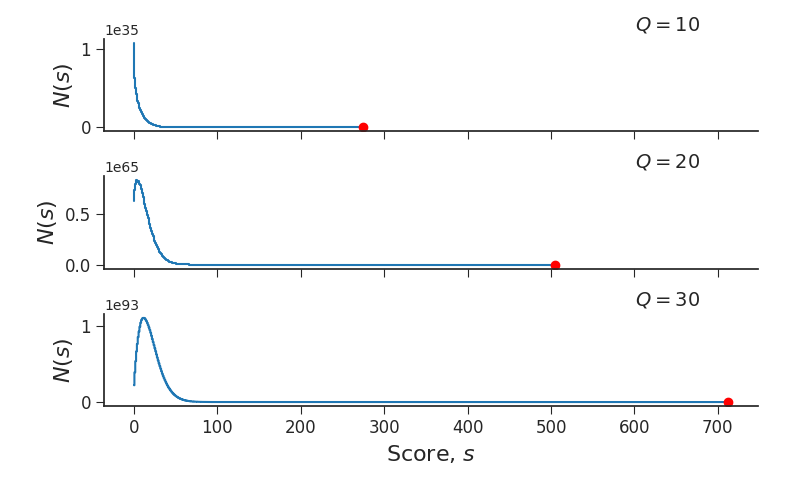
\includegraphics[width=.9\textwidth]{figures/score_distribuition_multiple.png}
    \end{center}
  \caption{{\bf Score distribution of a query size of 10, 20 and 30 genes against the ``Glycolysis/Gluconeogenesis'' pathway.} GeneSetDP enables us to calculate the full score distribution for a query of a given size, $Q$, i.e. how many ways one can reach a certain score when adding up the scores for $Q$ genes. A red dot marks the maximum score, $S$, for each case.}
  \label{fig:score_dist}
\end{figure}

\subsection*{Test of Calibration}

In order to test the statistical calibration of our method, we calculated $p$~values for 10000 random picks of gene sets of size $Q$ from the investigated genome using both GeneSetDP and GeneSetMC with $B = 100000$. As our selection is random and following our null hypothesis, we expected the resulting $p$~values to be uniformly distributed. To test this we plotted the $p$~values against their quantile in Fig \ref{fig:calibration} for $10000$ randomly assembled queries from the human genome. As a comparison, we also added a calibration curve for the popular NEA method BinoX\cite{ogris2016novel}. Here, for all three methods, we are only testing the queries for enrichment, that is, we are only concerned with a higher number of links than expected by random, and this differs from the default BinoX setting which tests for both enrichment and depletion. 
Also of note is the fact that, while we display all methods in the same figure, each represents its own calibration, and that the Spearman's correlation between BinoX and the other methods is fairly low ($\rho = 0.49$, $0.55$ and $0.55$ for $Q=10$, $20$ and $30$ respectively)

We note that the calibration of GeneSetDP is slightly conservative, i.e. the calculated $p$ values are larger than expected. Meanwhile, BinoX appears strongly anti-conservative, that is, the $p$ values are lower than expected.

\begin{figure}[htb]
  \begin{center}
		  \begin{tabular}[t]{c}
				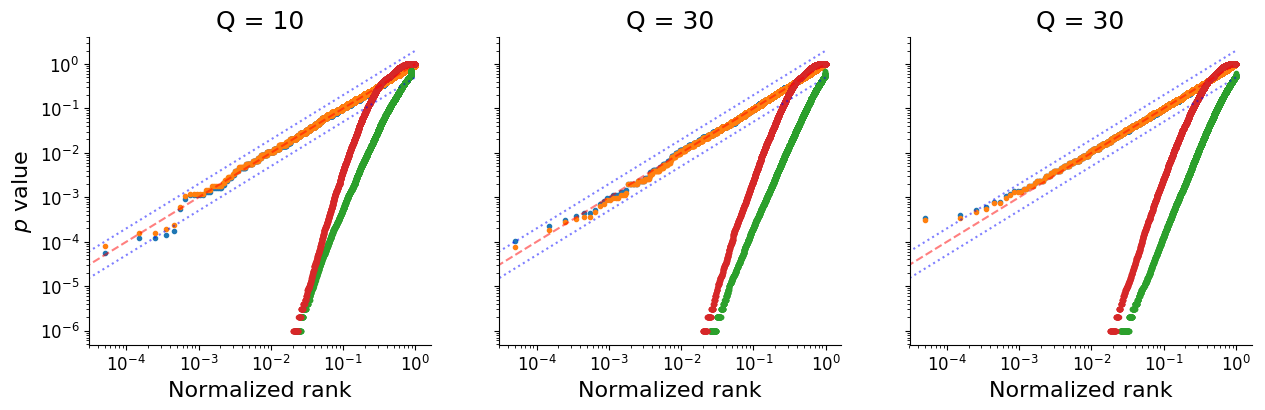
\includegraphics[width=.9\textwidth]{figures/calibration_multiple.png} \\
				
\includegraphics[width=0.45\textwidth]{figures/calibration_legend.png}
		\end{tabular}
  \end{center}
  \caption{{\bf Calibration of GeneSetDP and GeneSetMC.} We selected 10000 random sets of 10, 20 and 30 genes from the investigated genome definition and calculated their $p$ values with GeneSetMC and GeneSetDP against the ``Glycolysis/Gluconeogenesis'' pathway. To test the $p$~values uniformity we plotted them against their {\em normalized rank}, i.e. each $p$~value's (<rank>-0.5)/<total number of $p$~values>. We also added the calibration curve of BinoX, evaluated on the same random sets. The dashed line shows $y = x$ and the dotted lines $y = 2x$ and $y = 0.5x$, for comparison.}
  \label{fig:calibration}
\end{figure}

To test the consistency of the methods, we also investigated the correspondence between the $p$~values reported by GeneSetDP and GeneSetMC. As can be seen in Figure~\ref{fig:pscatter}, the results are consistent as expected.

\begin{figure}[htb]
  \begin{center}
		  \begin{tabular}[t]{c}
        % (Idea from reviewer comment in email 2018-06-08.)
				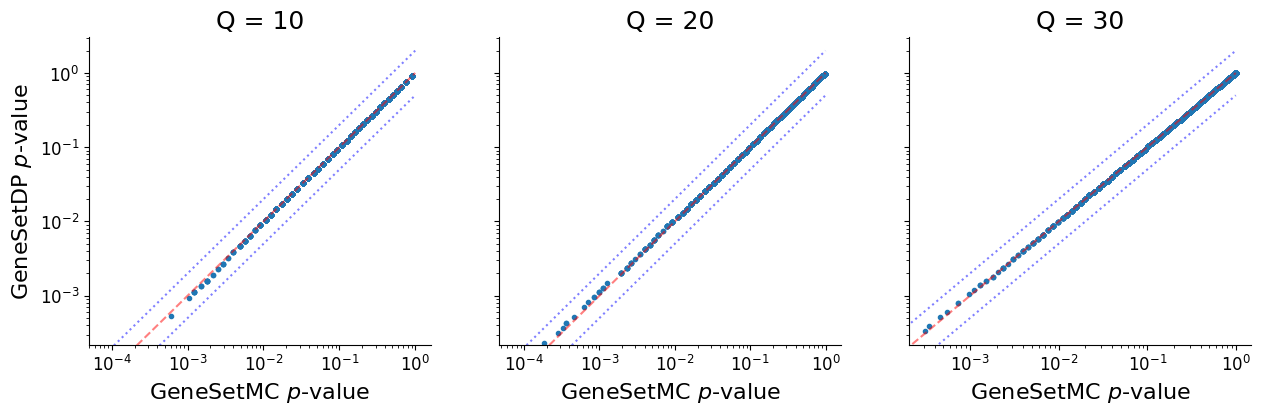
\includegraphics[width=.9\textwidth]{figures/scatter_dp_mc.png}
		\end{tabular}
  \end{center}
  \caption{{\bf Correspondence between GeneSetDP's and GeneSetMC's $p$~values.} We selected 10000 random sets of 10, 20 and 30 genes from the investigated genome definition and calculated their $p$ values with GeneSetMC and GeneSetDP against the ``Glycolysis/Gluconeogenesis'' pathway. We subsequently plotted the obtained $p$~values against each other. Again, the dashed line shows $y = x$ and the dotted lines $y = 2x$ and $y = 0.5x$.}
  \label{fig:pscatter}
\end{figure}



\section*{Discussion}

Here we have implemented two methods, GeneSetDP and GeneSetMC, to calculate unbiased $p$~values for inferences from NEA.
Instead of testing our methods' performance in terms of sensitivity, we here instead chose to test the method in terms of the methods statistical accuracy. We argue that more studies should make a point at demonstrating that their methods are well-calibrated, as it is a prerequisite for measuring performance at least when the ground truth of biological effect is not known.
With this in mind, we demonstrated that both our methods gave a better calibration than the popular BinoX method, by random sampling of subsets of a genome.

Both our implementations, GeneSetDP and GeneSetMC, are intended for measuring the enrichment of links between the query and the pathway set of genes. Most other NEA methods also report depletion of such links. One could easily modify our code to, instead of only measuring the higher scoring tail, measuring both tails of $N(s)$. However, this might result in a drop in sensitivity, so we have so far not implemented such a mechanism.

We made an explicit definition of the null hypothesis we employed, which centers on the query, $H_0$ : ``There are not more links between the query and pathway gene sets than expected by chance''. Previous implementations of NEA in the literature use Monte Carlo-simulation to determine parameters for various types parametric distributions, by perturbations of the investigated network. In practice, such perturbations are hard to conduct in a manner that they still resemble the original network, and hence are difficult to use to calculate accurate statistics. In general, it is easier to understand null models that relate to user actions, than more complex null models that relate to model parameters.

\section*{Acknowledgments}

LK was supported by a grant from the Swedish Foundation for Strategic Research (BD15-0043).

\bibliography{./refs.bib}

\end{document}
